\documentclass[11pt]{article}
\usepackage[margin=.8in]{geometry}
\usepackage{amsmath,amssymb,graphicx,hyperref}
\setlength{\parindent}{0pt}\setlength{\parskip}{7pt}
\begin{document}
\begin{center}{\Large Actual short residual certificate coverage}\\
23 November 2026 --- local unsigned Lean component evidence\end{center}
\textbf{Actual result.}
An explicit certificate consists of the actual affine target \(P\), a nonzero
actual coordinate function \(h\), an actual ideal \(J\), and at most two actual
nonsingular rational affine points \(Q_i\) in a fixed finite base \(B\), with
\[
 \langle h\rangle=I(P)^4J,\qquad
 J=\prod_{i:\operatorname{Fin}(n)}I(Q_i),\qquad n\le2.
\]
The empty product is the unit ideal. From these actual equalities, Lean derives
\(4P+\sum_iQ_i=0\), pads missing summands with the actual group identity, and
bounds the number of certified targets by \((|B|+1)^2\) when multiplication by
four is injective on those targets. If the actual finite group order is coprime
to four and \((|B|+1)^2\) is smaller than that order, an actual target lacks this
short certificate (PCC-20261123-89ca74) [pcc:unverified].

\begin{center}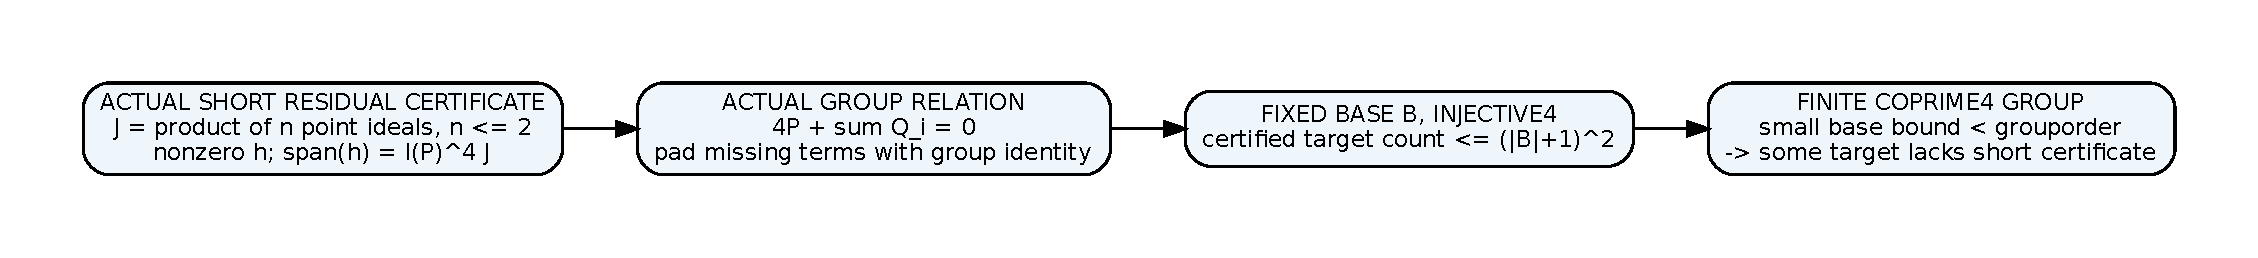
\includegraphics[width=\linewidth]{residual-short-dependencies-001.pdf}\end{center}

\textbf{Zero and one are explicit.}
The proof splits the actual \(n\le2\) into zero, one and two. Empty and
single-point sums use public finite-sum laws. Identity padding takes place in
the actual elliptic group; it does not invent an affine ideal at infinity.
The previous actual pair-image count applies to \(B\cup\{0\}\), whose cardinal
is at most \(|B|+1\) [pcc:unverified].

\textbf{Check and proof map.}
Source 078, build 084 and local receipt 041 check 200 local statements, three
new, exit zero, zero warnings, all printed foundations standard. The new
certificate definition and declarations are in the namespace below:
\begin{center}\begin{tabular}{l}
\texttt{OrientationActualResidualCoverage}\\
\texttt{short\_certificate\_padded\_relation}\\
\texttt{actual\_short\_certificate\_targets\_card}\\
\texttt{exists\_target\_without\_short\_certificate}
\end{tabular}\end{center}
PCC-20261123-89ca74 is unsigned local data outside the historical shared
Transport53/57 audit/fresh. Lean 4.35.0 and 255 input bindings are pinned.
Public finite-sum and finite-set cardinality results are reused; no new generic
law or arithmetic novelty is claimed [pcc:unverified].

\textbf{Scope and next test.}
Rational residual point factorization is an explicit certificate condition;
quotient dimension two does not imply it. This covers all zero/one/two rational
point-factor cases, including repeated points, for the stated fixed base and
injectivity premises. Nonsplit residue fields, adaptive or growing support,
known scalar extraction and full expected bit cost remain separate. Next bind
the actual residual fractional unit and class without assuming a rational
factorization, and test its dependence on the witness function.
\end{document}
